\chapter{Fluoride-Salt-Cooled High-Temperature Reactor Benchmark}
\label{chap:fhr-benchmark}
\acrfullpl{FHR} use \gls{TRISO} fuel and a low-pressure liquid fluoride-salt coolant.
\gls{FHR} technology combines \gls{FLiBe} coolant from \glspl{MSR} and 
\gls{TRISO} particles from \glspl{VHTR} to enable a reactor with 
low operating pressure, large thermal margin, and accident-tolerant 
qualities.
Within the \gls{FHR} reactor class, \glspl{AHTR} have plate-based fuel in a hexagonal 
fuel assembly. 
In section \ref{sec:fhr}, I gave an \gls{FHR} concept overview, 
an \gls{AHTR} design description, a review of previous efforts 
towards modeling these designs, and how these efforts led to the \gls{FHR} benchmark
initiation. 

To address the \gls{AHTR} modeling challenges, described in Chapter 
\ref{chap:lit-review}, such as multiple heterogeneity and material cross-section 
data, the \gls{OECD}-\gls{NEA} and \gls{Georgia Tech} initiated the \gls{FHR} 
benchmark for the \gls{AHTR} design in 2019 \cite{petrovic_benchmark_2021}. 
\gls{UIUC} participates in the benchmark with the OpenMC Monte Carlo code 
\cite{romano_openmc_2013} using the ENDF/B-VII.1 material cross section library 
\cite{chadwick_endf/b-vii.1_2011}.
The \gls{UIUC} team consists of myself and my advisors, Professor Kathryn Huff and Dr
Madicken Munk. 

The three-phase \gls{FHR} benchmark begins with a single fuel assembly 
simulation without burnup and gradually extends to full core depletion. 
Table \ref{tab:phases} outlines the complete and incomplete benchmark phases.
\begin{table}[htbp]
    \centering
    \onehalfspacing
    \caption{\acrfull{OECD} \acrfull{NEA} \acrfull{FHR} benchmark Phases 
    \cite{noauthor_fluoride_nodate}.}
	\label{tab:phases}
    \footnotesize
    \begin{tabular}{lclc}
    \hline 
    \textbf{Phases}& \textbf{Sub-phases} & \textbf{Description} & \textbf{Completed?} \\
    \hline
    \multirow{ 3}{5cm}{\textbf{Phase I: fuel assembly}} & I-A & 2D model, steady-state & \checkmark\\
    &I-B & 2D model depletion & \checkmark\\
    &I-C & 3D model depletion &\\
    \hline
    \multirow{2}{5cm}{\textbf{Phase II: 3D full core}}&II-A & Steady-state &\\
    &II-B & Depletion &\\
    \hline 
    \multirow{ 2}{5.5cm}{\textbf{Phase III: 3D full core with feedback \& multicycle analysis}}&III-A & Full core depletion with feedback &\\
    &III-B & Multicycle analysis &\\
    \hline
    \end{tabular}
\end{table}

In the subsequent sections, I will describe the benchmark's specifications for 
the \gls{AHTR} design and Phase I. Then, I will share our Phase I-A and I-B 
results generated with the OpenMC neutronics code \cite{romano_openmc_2013}. 
And finally, preliminary \gls{AHTR} multiphysics simulation results.  

\section{FHR Benchmark \acrlong{AHTR} Design}
Figure \ref{fig:reactor-schematic} shows the \acrfull{AHTR} schematic and a vertical 
cut of the reactor vessel. 
The \gls{AHTR} operates at 3400 MWt thermal power and 1400 MWe 
electric power \cite{varma_ahtr_2012}. 
\begin{figure}[htbp]
    \centering
    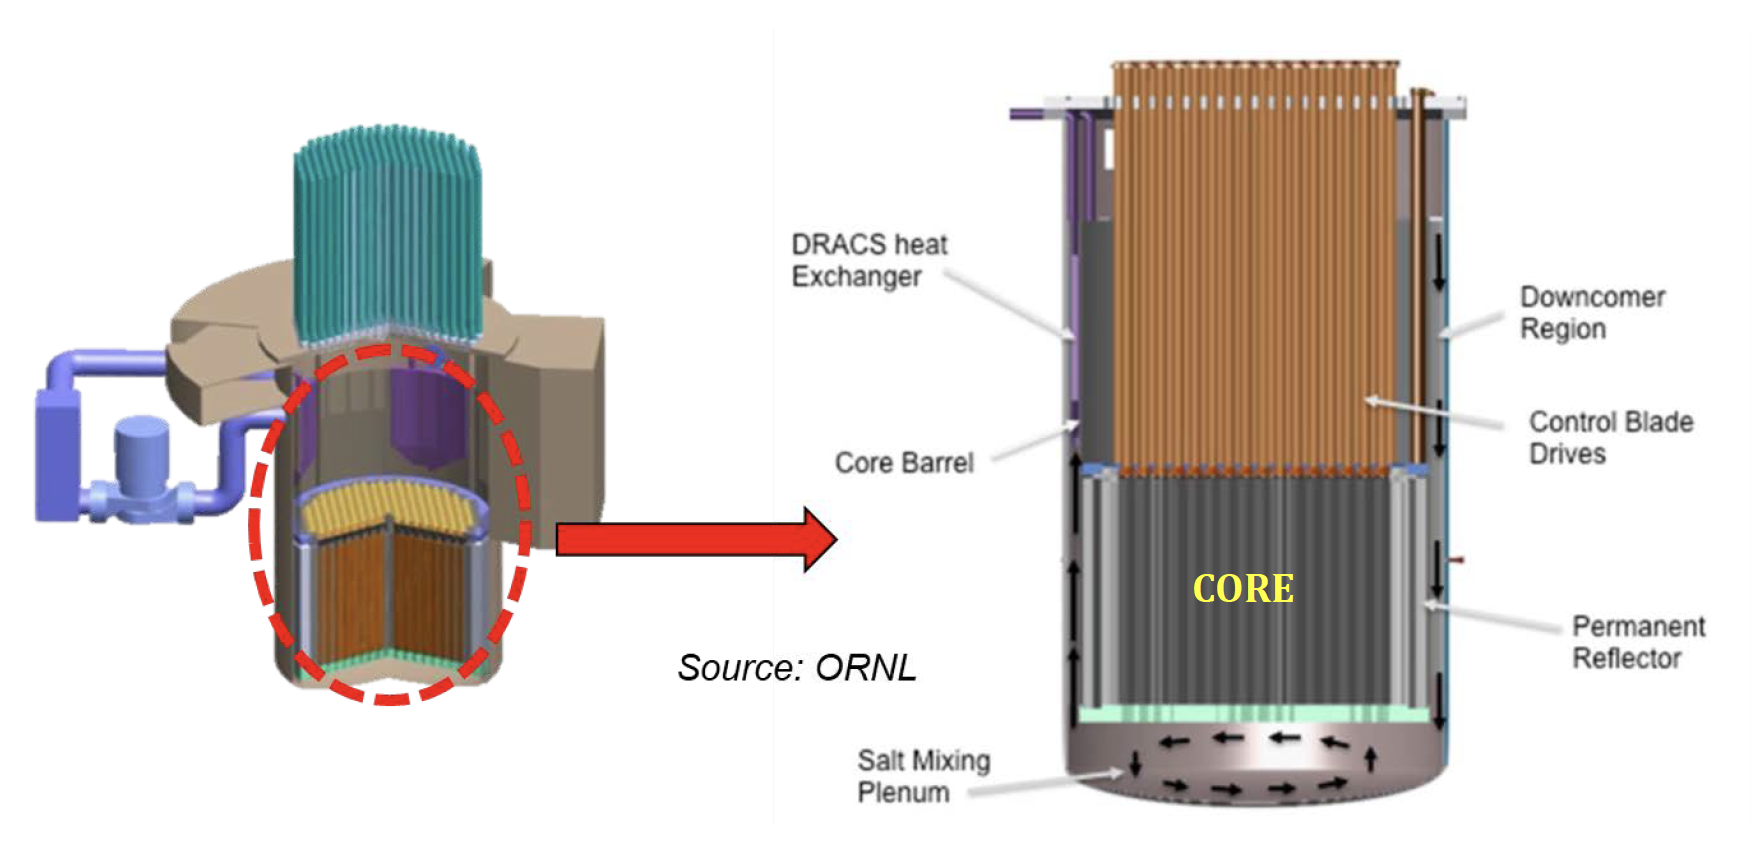
\includegraphics[width=\linewidth]{reactor-schematic.png} 
    \caption{\acrfull{AHTR} schematic (left) and vessel (right) reproduced from
    \cite{petrovic_benchmark_2021}.}
    \label{fig:reactor-schematic}
\end{figure}
The $10m$-diameter exterior reactor vessel contains an $8m$-diameter 
reactor core that which in turn contains 252 hexagonal fuel assemblies.

Each $6m$ high fuel assembly comprises a $5.5m$ active core region, which contains
\gls{TRISO} particles, and $0.25m$ top and bottom non-fuelled reflector regions.
Figure \ref{fig:ahtr}, from Chapter \ref{chap:lit-review}, shows a single 
hexagonal fuel assembly geometry and the arrangement of all assemblies in the core.
All dimensions specified are at room temperature. 
The benchmark's phases I and II use room temperature dimensions while phase III 
will address dimensional changes brought about by temperature expansion. 
Figure \ref{fig:ahtr-fuel-assembly} shows a detailed 2D view of the 
\gls{AHTR}'s hexagonal fuel assembly. 
\begin{figure}[htbp]
    \centering
    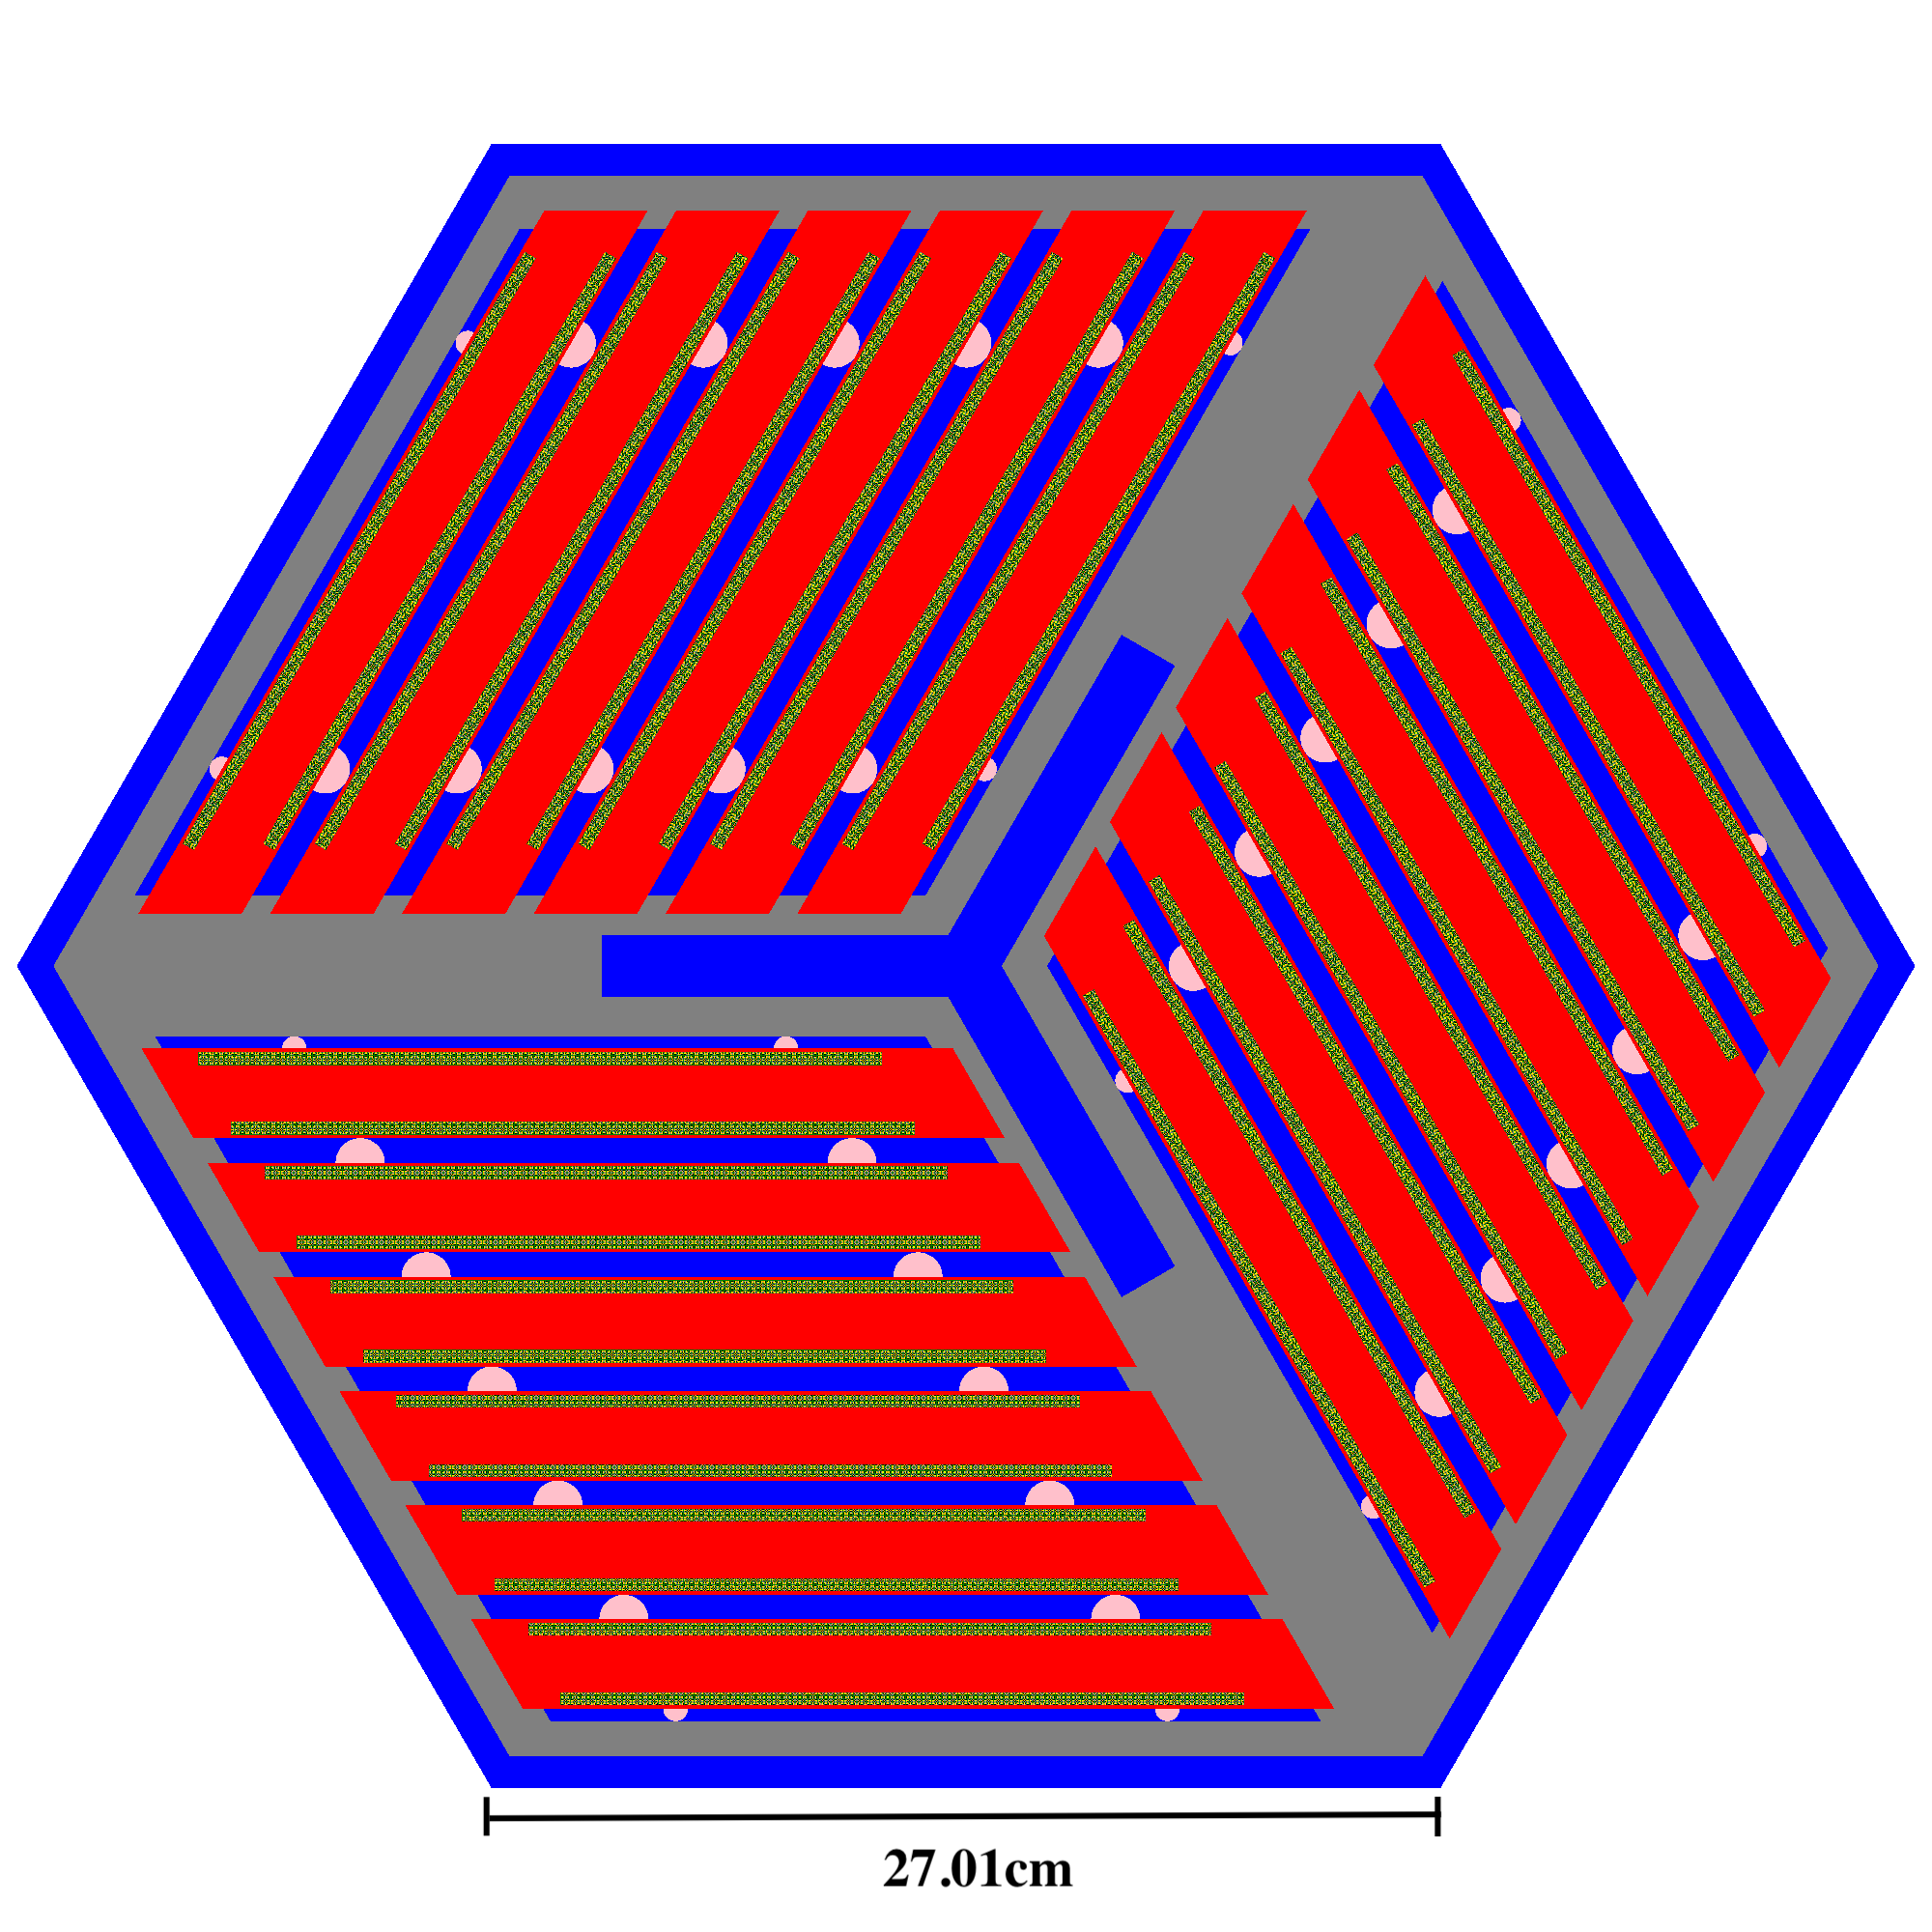
\includegraphics[width=0.9\linewidth]{ahtr-fuel-element.png} 
    \resizebox{0.4\textwidth}{!}{
        \fbox{\begin{tabular}{ll}
            \textcolor{fhrblue}{$\blacksquare$} & FLiBe \\
            \textcolor{fhrgrey}{$\blacksquare$} & Graphite (Fuel Structure)\\
            \textcolor{fhrred}{$\blacksquare$} & Graphite (Fuel Plank) \\
            \textcolor{fhrpink}{$\blacksquare$} & Graphite (Spacers) \\
            \textcolor{fhrgreen}{$\blacksquare$} & Graphite (Fuel Stripe) \\
            \textcolor{fhryellow}{$\blacksquare$} & TRISO particle \\
            \end{tabular}}}
            \hspace{0.5cm}
            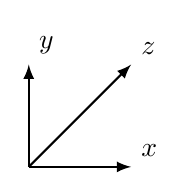
\begin{tikzpicture}
                \draw[ thick,-latex] (0,0) -- (1.3,0) node[anchor=south west] {$x$};
                \draw[ thick,-latex] (0,0) -- (0,1.3) node[anchor=south west] {$y$};
                \draw[ thick,-latex] (0,0) -- (1.3,1.3) node[anchor=south west] {$z$};
               \tkzText[above](-0.5,1){}
               \end{tikzpicture} 
    \caption{\acrfull{AHTR} fuel assembly with 18 fuel plates arranged in 
    three diamond-shaped sectors, with a central Y-shaped and external channel 
    graphite structure.}
    \label{fig:ahtr-fuel-assembly}
\end{figure}
The hexagonal fuel assembly consists of eighteen fuel-containing graphite planks 
arranged in three diamond-shaped sectors, with a external channel wrapper and 
structural Y-shape, made of C-C composite with extra notches to hold the fuel 
planks in place. 
The diamond-shaped sections have $120^\circ{}$ rotational symmetry with each other 
\cite{varma_ahtr_2012,ramey_monte_2018,petrovic_benchmark_2021}. 
Semi-cylindrical graphite spacers attach to the fuel planks with radius equalling to 
coolant channel thickness. 
\gls{FLiBe} coolant fills the gaps between the fuel planks, and between 
assemblies (note: FliBe layer around the single assembly). 
The Y-shaped control rod slot at the center of the Y-shape structure contains 
\gls{FLiBe} coolant when the control blade is not in the slot (as seen in 
Figure \ref{fig:ahtr-fuel-assembly})
\cite{varma_ahtr_2012,ramey_monte_2018,petrovic_benchmark_2021}.
For a single fuel assembly, the internal $120^\circ{}$ rotational symmetry is 
represented by periodic boundary conditions, as seen in Figure \ref{fig:bc}. 
\begin{figure}[htbp]
    \centering
    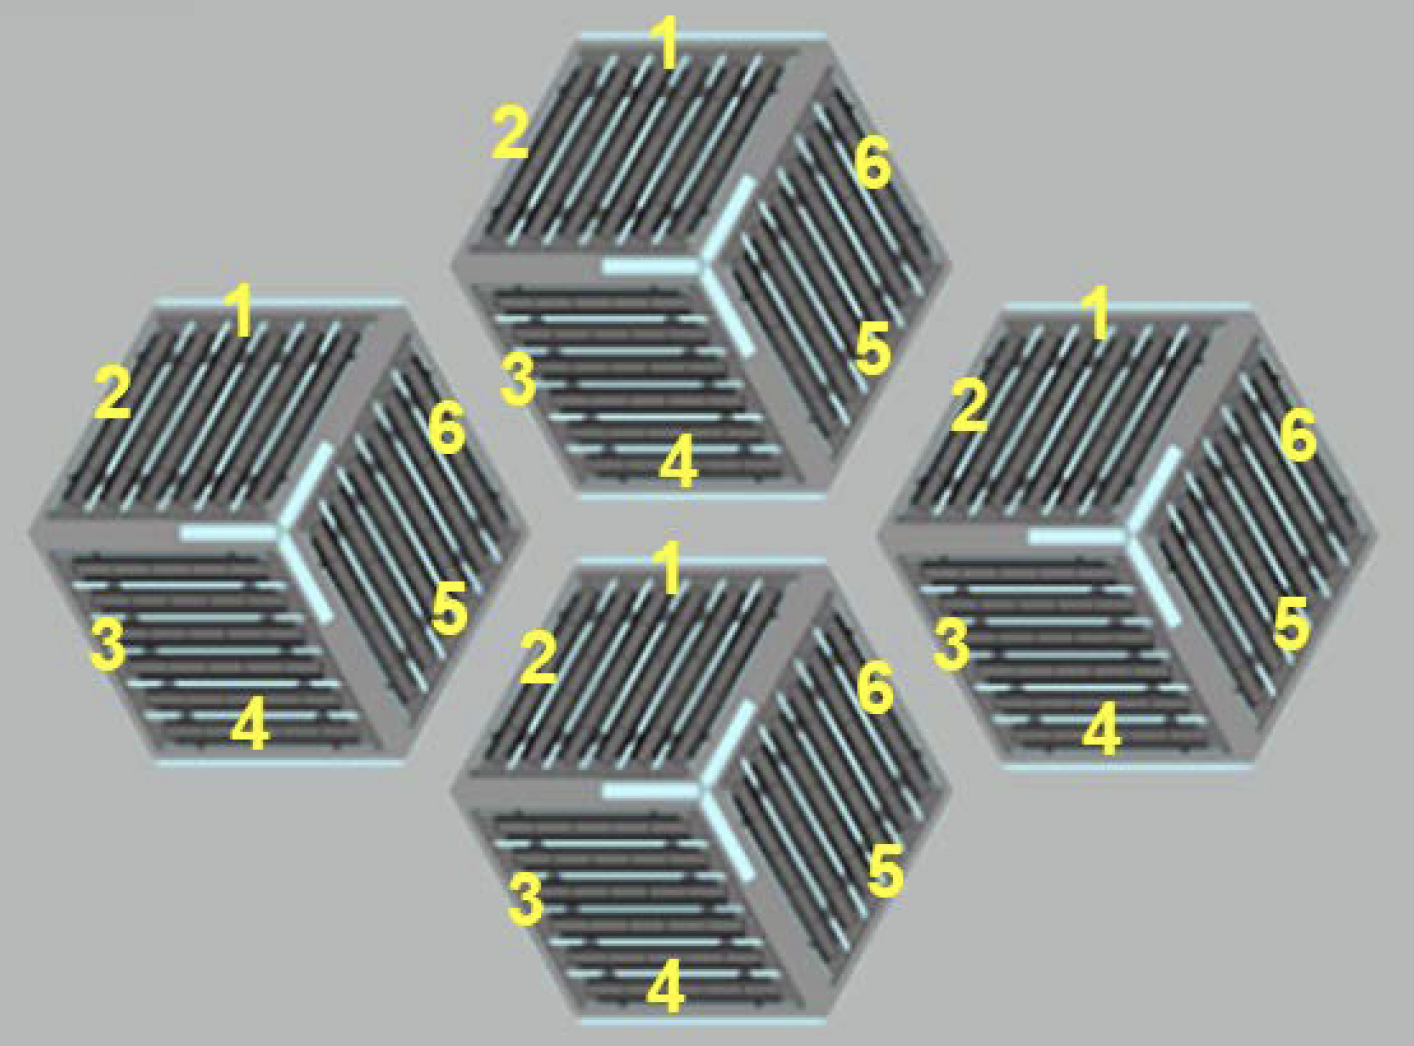
\includegraphics[width=0.72\linewidth]{bc.png} 
    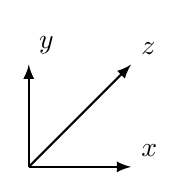
\begin{tikzpicture}
        \draw[ thick,-latex] (0,7) -- (1.3,7) node[anchor=south west] {$x$};
        \draw[ thick,-latex] (0,7) -- (0,8.3) node[anchor=south west] {$y$};
        \draw[ thick,-latex] (0,7) -- (1.3,8.3) node[anchor=south west] {$z$};
       \tkzText[above](-0.5,0){}
       \end{tikzpicture} 
    \caption{Visualization of periodic boundary conditions for a single fuel 
    assembly in the \acrfull{AHTR}, reproduced from \cite{petrovic_benchmark_2021}.}
    \label{fig:bc}
\end{figure}

Figure \ref{fig:ahtr-fuel-plank} magnifies a single fuel plank. 
Fuel stripes line the upper and lower sides of each graphite fuel plank. 
\begin{figure}[htbp]
    \centering
    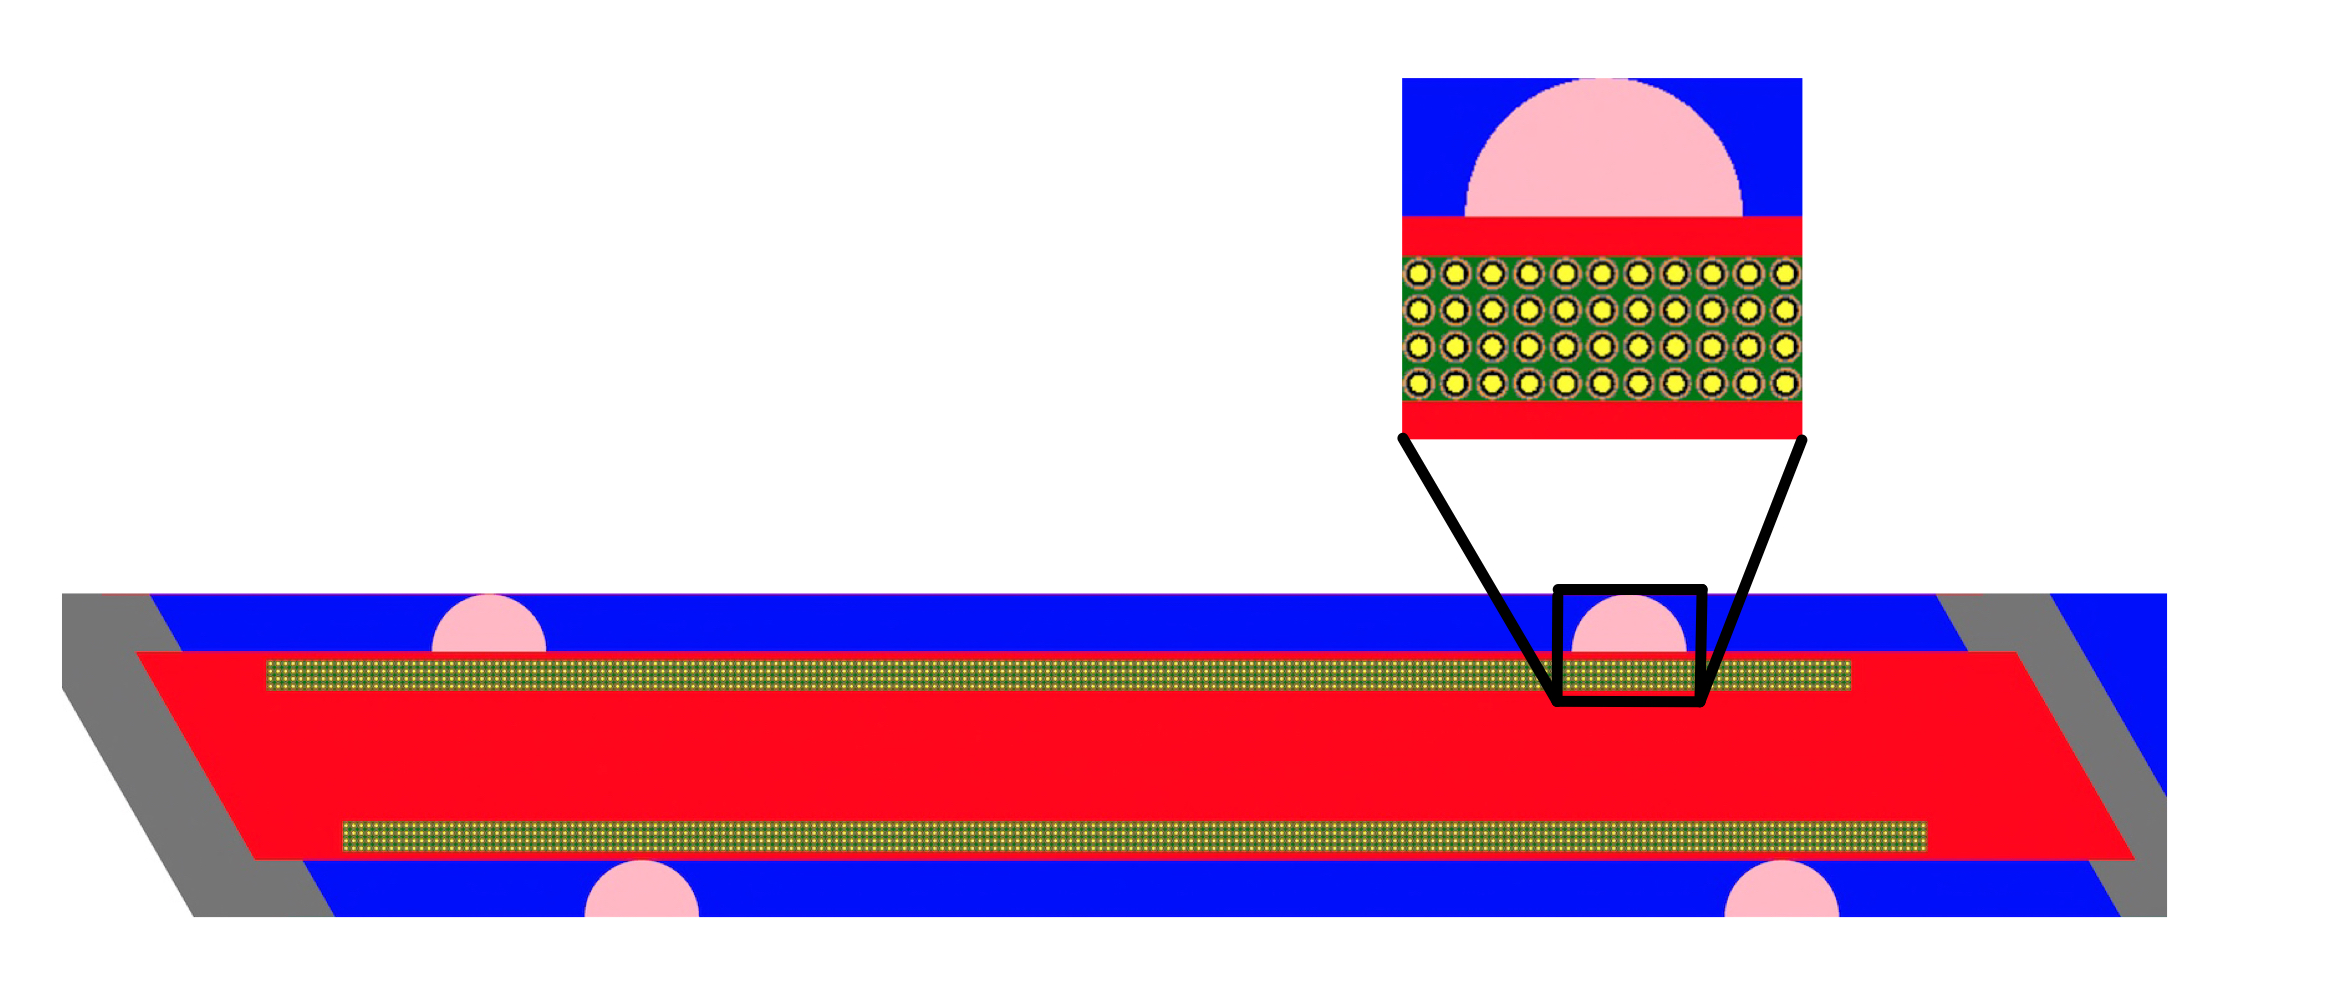
\includegraphics[width=\linewidth]{ahtr-fuel-plank.png} 
    \resizebox{0.4\textwidth}{!}{
        \fbox{\begin{tabular}{ll}
            \textcolor{fhrblue}{$\blacksquare$} & FLiBe \\
            \textcolor{fhrgrey}{$\blacksquare$} & Graphite (Fuel Structure)\\
            \textcolor{fhrred}{$\blacksquare$} & Graphite (Fuel Plank) \\
            \textcolor{fhrgreen}{$\blacksquare$} & Graphite (Fuel Stripe) \\
            \textcolor{fhryellow}{$\blacksquare$} & TRISO particle \\
            \textcolor{fhrpink}{$\blacksquare$} & Graphite (Spacer) \\
            \end{tabular}}}
            \hspace{0.5cm}
            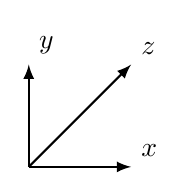
\begin{tikzpicture}
                \draw[ thick,-latex] (0,0) -- (1.3,0) node[anchor=south west] {$x$};
                \draw[ thick,-latex] (0,0) -- (0,1.3) node[anchor=south west] {$y$};
                \draw[ thick,-latex] (0,0) -- (1.3,1.3) node[anchor=south west] {$z$};
               \tkzText[above](-0.5,1){}
               \end{tikzpicture} 
    \caption{\acrfull{AHTR}'s fuel plank, with the magnification of 
    a spacer and segment of the fuel stripe with embedded \gls{TRISO} particles.}
    \label{fig:ahtr-fuel-plank}
\end{figure}
Each fuel stripe contains a graphite matrix filled with a cubic lattice of 
\gls{TRISO} particles with 40\% packing fraction. 
The lattice is 210 \gls{TRISO} particles wide in the x-direction, four particles 
deep in the y-direction, and 5936 particles tall in the z-direction. 
Figure \ref{fig:ahtr-triso} shows the \gls{TRISO} particle's cross section 
which consists of five layers: oxycarbide fuel kernel, porous carbon buffer, 
inner pyrolytic carbon, silicon carbide layer, and the outer pyrolitic carbon. 
\begin{figure}[htbp]
    \centering
    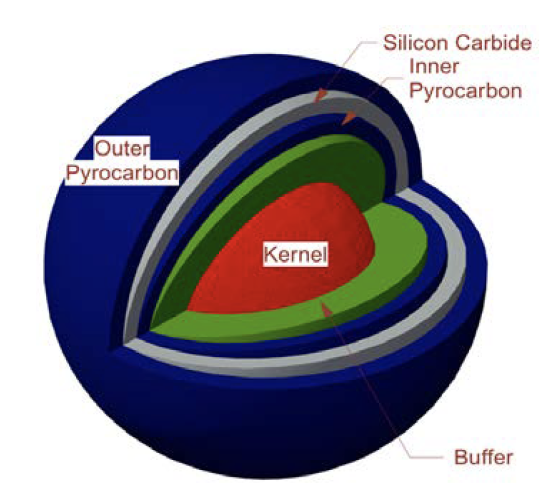
\includegraphics[width=0.6\linewidth]{ahtr-triso.png} 
    \caption{\acrlong{AHTR}'s TRISO particle schematic reproduced from 
    \cite{petrovic_benchmark_2021}.}
    \label{fig:ahtr-triso}
\end{figure}

To control reactivity, the \gls{FHR} benchmark includes \gls{AHTR} configurations
with burnable poisons and control rods. 
The burnable poisons consist of europium oxide, $Eu_2O_3$, and have a discrete
or integral (dispersed) option. 
Figure \ref{fig:discrete-poison} shows the discrete option with z-direction axially 
stacked small spherical $Eu_2O_3$ particles at five XY locations in each 
fuel plank. 
\begin{figure}[htbp]
    \centering
    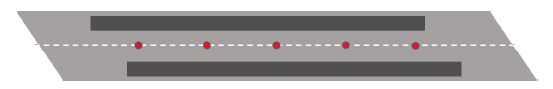
\includegraphics[width=0.82\linewidth]{discrete-poison.png}
    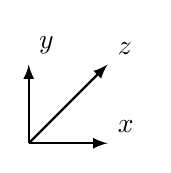
\begin{tikzpicture}
        \draw[ thick,-latex] (0,0) -- (1,0) node[anchor=south west] {$x$};
        \draw[ thick,-latex] (0,0) -- (0,1) node[anchor=south west] {$y$};
        \draw[ thick,-latex] (0,0) -- (1,1) node[anchor=south west] {$z$};
       \tkzText[above](-0.3,-0.7){}
       \end{tikzpicture} 
    \caption{XY Placement of z-direction axial burnable poisons stacks in the \acrlong{AHTR} 
    \cite{noauthor_fluoride_nodate}.}
    \label{fig:discrete-poison}
\end{figure}
The integral options consists of $Eu_2O_3$ homogenously mixed with the graphite 
fuel plank (including the graphite in fuel stripes matrix and plank ends 
indented to structural sides, but excluding the graphite in spacers and 
graphite in TRISO particles).
The \gls{MHC} control rod inserts into the Y-shaped control rod slot where it 
displaces the \gls{FLiBe} that occupies the slot 
(shown in Figure \ref{fig:ahtr-fuel-assembly}). 

\section{FHR Benchmark Phase I Specifications}
\label{sec:phase1}
The \gls{FHR} benchmark Phase I consists of three subphases.
First, a steady-state 2D model (Phase I-A), next depletion of one 2D \gls{FHR} fuel 
assembly (Phase I-B), and finally depletion of one 3D \gls{FHR} fuel assembly 
(Phase I-C).
Benchmark organizers have only released Phase I-A and I-B's specifications, thus 
Phase I-C's specifications will be omitted in this section.

The benchmark requires the following results for Phases I-A and I-B:
\begin{enumerate}[label=(\alph*)]
    \item $k_{eff}$ (effective multiplication factor)
    \item reactivity coefficients: $\beta_{eff}$ (effective delayed neutron fraction), 
    $\alpha_D$ (doppler coefficient), $\alpha_{T, FliBe}$ (\gls{FLiBe} temperature 
    coefficient), $\alpha_{M}$ (moderator temperature coefficient)
    \item tabulated fission source distribution by one-fifth fuel stripe
    \item $\bar{\phi_1}, \bar{\phi_2}, \bar{\phi_3}$ (neutron flux averaged over 
    the whole model tabulated in three coarse energy groups)
    \item $\phi_1(\vec{x},\vec{y}), \phi_2(\vec{x},\vec{y}), \phi_3(\vec{x},\vec{y})$ 
    (neutron flux distribution in three coarse energy groups) 
    \item fuel assembly averaged neutron spectrum
\end{enumerate}
Next, I report the equations used to calculate these required results.  

\subsubsection{Reactivity Coefficients (b)}
I assumed one energy group and six delayed groups for $\beta_{eff}$. 
Reactivity coefficient, $\alpha$, is the change in reactivity ($\rho$) of the 
material per degree change in the material's temperature (T). 
I calculated each reactivity coefficient and its corresponding uncertainty 
with these equations: 
\begin{align}
    \label{eq:reactivity-coefficient}
    \frac{\Delta \rho}{\Delta T} &= 
    \frac{\rho_{T_{high}}-\rho_{T_{low}}}{T_{high}-T_{low}} \ [\frac{pcm}{K}] \\
    \delta \frac{\Delta \rho}{\Delta T} &= 
    \frac{\sqrt{\delta (\rho_{T_{high}})^2+(\delta \rho_{T_{low}})^2}}{T_{high}-T_{low}} \ [\frac{pcm}{K}] 
\end{align}

\subsubsection{Fission Source Distribution / Fission Density (c)}
I calculated \gls{FD} with OpenMC's \texttt{fission} tally score (f) 
for each region divided by the average \texttt{fission} tally score of all the regions:
\begin{align}
    FD_i &=  \frac{f_i}{f_{ave}}\ [-]\\
    \intertext{where}
    f_i &= \mbox{fission reaction rate in a single region i [reactions/src]} \nonumber \\
    f_{ave} &= \mbox{average of all $f_i$ [reactions/src]} \nonumber
\end{align}
The uncertainty calculations for $FD_i$ and $f_{ave}$: 
\begin{align}
    \delta FD_i &= |FD_i| \sqrt{\left(\frac{\delta f_i}{f_i}\right)^2+\left(\frac{\delta f_{ave}}{f_{ave}}\right)^2} \\
    \delta f_{ave} &= \frac{1}{N}\sqrt{\sum_i^Nf_i^2} \\
    \intertext{where}
    N &= \mbox{No. of fission score values} \nonumber
\end{align}

\subsubsection{Neutron Flux (d, e, f)}
OpenMC's \texttt{flux} score is normalized per source particle simulated, resulting 
in [$\frac{neutrons\ cm}{src}$] units.
This is an unnatural unit for system analysis, and thus to better compare OpenMC
results with other software results in the benchmark, I converted flux to 
[$\frac{neutrons}{cm^2s}$] units using the following equations:  
\begin{align}
    \Phi_c &= \frac{N \cdot \Phi_o}{V} \\
    N &= \frac{P\cdot\nu}{Q\cdot k} \\
    \intertext{where}
    \Phi_c &= \mbox{converted flux [$\frac{neutrons}{cm^2s}$]} \nonumber \\ 
    \Phi_o &= \mbox{original flux [$\frac{neutrons\ cm}{src}$]} \nonumber \\
    N &= \mbox{normalization factor [$\frac{src}{s}$]} \nonumber \\
    V &= \mbox{volume of fuel assembly [$cm^3$]} \nonumber \\
    P &= \mbox{power [$\frac{J}{s}$]} \nonumber \\
    \nu &= \mbox{$\frac{\nu_f}{f}$ [$\frac{neutrons}{fission}$]} \nonumber \\
    Q &= \mbox{Energy produced per fission [$\frac{J}{fission}$]} \nonumber \\
    &= \mbox{$3.2044 \times 10^{-11}$ J per $U_{235}$ fission} \nonumber \\
    k &= \mbox{$k_{eff}$ [$\frac{neutrons}{src}$]} \nonumber 
\end{align}
The flux standard deviation is: 
\begin{align}
    \delta \Phi_c = \Phi_c \times
    \sqrt{(\frac{\delta \Phi_o}{\Phi_o})^2+ (\frac{\delta \nu_f}{\nu_f})^2 
    + (\frac{\delta k}{k})^2 + (\frac{\delta f}{f})^2}
\end{align}
I calculated reactor power based on the given reference specific power 
($P_{sp}$) of 200 $\frac{W}{gU}$: 
\begin{align}
    P &= P_{sp} \times V_F \times \rho_F \times \frac{wt\%_{U}}{100} \\
    \intertext{where}
    V_F &= \mbox{volume of fuel [$cm^3$]} \nonumber \\ 
    &= \frac{4}{3} \pi r_f^3 \times N_{total} \nonumber \\
    r_f &= \mbox{radius of fuel kernel within TRISO particl [cm]} \nonumber\\
    N_{total} &= \mbox{total no. of TRISO particles in fuel assembly} \nonumber \\ 
    &= 101 \times 210 \times 4 \times 2 \times 6 \times 3 \nonumber\\ 
    \rho_F &= \mbox{density of fuel [$g/cc$]} \nonumber \\
    wt\%_{U} &= \frac{at\%_{U235} \times m_{U235} + at\%_{U238} \times m_{U238}}{\sum (at\%_i \times m_i)} \times 100 \nonumber\\
    m &= \mbox{atomic mass} \nonumber
\end{align}

\subsection{Phase I-A Specifications}
For Phase I-A, the benchmark specifies that each participant must produce a 
steady-state 2D model of one fresh fuel assembly for nine cases
and report the required results listed in Section \ref{sec:phase1}.  
Table \ref{tab:phase1a-cases} describes each case. 
\begin{table}[htbp]
    \centering
    \onehalfspacing
    \caption{Description of the \acrlong{FHR} benchmark Phase I-A cases \cite{noauthor_fluoride_nodate}.}
	\label{tab:phase1a-cases}
    \footnotesize
    \begin{tabular}{p{0.05\textwidth}p{0.95\textwidth}}
    \hline 
    \textbf{Case} & \textbf{Description} \\
    \hline
    1A & Reference case. Hot full power (HFP), with temperatures of 1110K for 
    fuel kernel and 948K for coolant and all other materials (including TRISO 
    particle layers other than fuel kernel). Nominal (cold) dimensions, 
    9 wt\% enrichment, no \acrlong{BP}, \acrlong{CR} out.\\
    \hline
    2AH & \Gls{HZP} with uniform temperature of 948 K, 
    otherwise same as Case 1A. Comparison with Case 1A provides HZP-to-HFP power 
    defect.\\
    \hline 
    2AC & \Gls{CZP}. Same as Case 2AH, but with uniform temperature 
    of 773 K. Comparison with Case 2AH provides isothermal temperature coefficient.\\
    \hline
    3A & \Acrlong{CR} inserted, otherwise same as Case 1A. \\
    \hline
    4A & Discrete europia \acrlong{BP}, otherwise same as Case 1A.\\
    \hline
    4AR & Discrete europia \acrlong{BP} and \acrlong{CR} inserted, otherwise same as 
    Case 1A. \\
    \hline
    5A & Integral (dispersed) europia \acrlong{BP}, otherwise same as Case 1A. \\
    \hline
    6A & Increased \gls{HM} loading (4 to 8 layers of \gls{TRISO}) decreased C/HM 
    ratio (from about 400 to about 200) and decreased specific power to 100 W/gU, 
    otherwise same as Case 1A.\\
    \hline 
    7A & Fuel enrichment 19.75 wt\%, otherwise same as Case 1A.\\
    \hline 
    \end{tabular}
\end{table}

\subsection{Phase I-B Specifications}
For Phase I-B, the benchmark specifies that each participant must produce 
depletion results for three cases: 1B, 4B, and 7B. 
These are the same as cases 1A, 4A, and 7A (described in Table \ref{tab:phase1a-cases}), 
but with depletion steps added. 
The depletions steps are 0, 0.1, 0.5, 1, 2, 4, 6, 8, 10, 14, 18, 22, 26, 30, 40, 50, 
60, 70 GWd/tU. 
Case 7B adds seven more depletion steps: 80, 90, 100, 120, 140, 160 GWd/tU. 
The benchmark assumes that depletion occurs only in the fuel and burnable poisons 
and that the depletion performs under the critical spectrum assumption. 

\section{FHR Benchmark Phase I Results}
The \texttt{arfc/fhr-benchmark} Github repository contains all the results submitted 
by \gls{UIUC} for the \gls{FHR} benchmark \cite{chee_arfcfhr-benchmark_2021}. 
The benchmark used a phased blind approach -- participants were asked to 
submit Phase I-A and I-B results without knowledge of other submissions. 
Petrovic et al. \cite{petrovic_preliminary_2021} describes the preliminary 
results of the benchmark across several institutions and concludes 
that the overall observed agreement is satisfactory. 
In the subsequent sections, I will share the results obtained by \gls{UIUC}. 

\subsection{Results: Phase I-A}
In a recently submitted \gls{ANS} Mathematics \& Computation (M$\&$C) 2021 conference paper 
(which I am a co-author on), Petrovic et al. \cite{petrovic_preliminary_2021} compared 
\gls{FHR} benchmark participants' Phase I-A $k_{eff}$ results.  
We reported that the standard deviation between participants for each case 
was in the 231 to 514 pcm range, acceptable and notably close given a blind 
benchmark, assuring that \gls{UIUC}'s Phase I-A results are acceptable and 
in agreement with other benchmark participants. 

\subsubsection{Results: Effective Multiplication Factor (a)}
Table \ref{tab:phase1a-results} reports Phase I-A $k_{eff}$ results. 
I ran the simulations on \gls{UIUC}'s BlueWaters supercomputer with 64 XE nodes, 
which each have 32 cores \cite{ncsa_about_2017}. 
To reduce the statistical uncertainty of $k_{eff}$ to $\sim$10pcm, I ran each 
simulation with 500 active cycles, 100 inactive cycles, and 200000 neutrons. 
Each simulation took \gls{WCT} ranging from 2 to 5 hours. 
\begin{table}[htbp]
    \centering
    \onehalfspacing
    \caption{\acrlong{UIUC}'s \acrlong{FHR} Benchmark Phase I-A results 
    \cite{chee_arfcfhr-benchmark_2021}.}
	\label{tab:phase1a-results}
    \footnotesize
    \begin{tabular}{cp{2.7cm}cccccc}
    \hline
    \textbf{Case} & \textbf{Summary} & \textbf{WCT [hr]} & \textbf{$k_{eff}$}* & 
    \textbf{$\beta_{eff}$}** & 
    \textbf{Fuel} $\frac{\Delta \rho}{\Delta T}$ & 
    \textbf{FliBe} $\frac{\Delta \rho}{\Delta T}$ & 
    \textbf{Graphite} $\frac{\Delta \rho}{\Delta T}$\\
    \hline 
    1A & Reference &2.82&1.39389 & 0.006534 & -2.24$\pm$0.15 & -0.15$\pm$0.15 & -0.68$\pm$0.15\\
    2AH & \gls{HZP} &2.82&1.40395 & 0.006534 & -3.14$\pm$0.15 & -0.20$\pm$0.14 & -0.85$\pm$0.14\\
    2AC & \gls{CZP} &2.75&1.41891 & 0.006534 & -3.36$\pm$0.14 & -0.11$\pm$0.14 & 0.07$\pm$0.14\\
    3A & CR &2.49&1.03147 & 0.006534 & -4.03$\pm$0.28 & -0.83$\pm$0.27 & -3.18$\pm$0.29\\
    4A & Discrete BP &5.08&1.09766 & 0.006542 & -4.06$\pm$0.24 & -1.55$\pm$0.23 & -6.51$\pm$0.24\\
    4AR & Discrete BP + CR &4.59&0.84158 & 0.006553 & -5.60$\pm$0.49 & -1.78$\pm$0.46 & -10.44$\pm$0.47\\
    5A & Dispersed BP &2.33&0.79837 & 0.006556 & -5.09$\pm$0.40 & -4.87$\pm$0.40 & -22.99$\pm$0.38\\
    6A & Increased \gls{HM} &3.52&1.26294 & 0.006556 & -4.46$\pm$0.19 & 0.16$\pm$0.20 & -0.39$\pm$0.20\\
    7A & 19.75\% Enriched &2.21&1.50526 & 0.006530 & -2.49$\pm$0.13 & -0.12$\pm$0.12 & -0.62$\pm$0.12\\
    \hline
    \multicolumn{5}{l}{BP: burnable poison, CR: control rod} \\
    \multicolumn{5}{l}{* All $k_{eff}$ values have an uncertainty of 0.00010.} \\
    \multicolumn{5}{l}{** All $\beta_{eff}$ values have an uncertainty of 0.000001.}
    \end{tabular}
\end{table}

Cases 2AH and 2AC are at zero power, meaning that the fuel assembly is exactly 
critical but not producing any energy. 
For both cases, $k_{eff}$ is higher than the reference Case 1A, which I attribute to 
lower fuel temperatures. 
At lower fuel temperatures, less doppler broadening occurs, resulting in less neutron 
capture, thus, increasing $k_{eff}$. 
As expected, $k_{eff}$ is lower for Cases 3A, 4AR, and 5A than reference case 
1A since these cases introduce burnable poisons and control rods to the fuel 
assembly. 
Also, as expected, $k_{eff}$ is higher for Case 7A than reference Case 1A, since 
it has a higher enrichment. 
However, Case 6A deviated from expectations with a lower $k_{eff}$ despite an increase 
in \acrlong{HM} loading. 
This behavior is due to reduced moderation and worsened fuel utilization brought about 
by self-shielding, demonstrating that an increase in fuel packing fraction does not 
always correspond with an increased $k_{eff}$. 

\subsubsection{Results: Reactivity Coefficients (b)}
Table \ref{tab:phase1a-results} reports Phase I-A reactivity coefficients results. 
$\beta_{eff}$ increased by 10--20[pcm] for Cases 4A, 4AR, 5A, and 6A compared to
reference Case 1A due to the introduction of control rods and poisons that 
shift the average neutron velocity to higher values, resulting in decreased
thermal fission and increased fast fission \cite{torabi_neutronic_2018}.
In Table \ref{tab:phase1a-results},most temperature coefficients are negative, 
exemplifying the \gls{AHTR}'s passive safety behavior. 
Negative reactivity feedback results in a self-regulating reactor; if the reactor 
power rises, resulting in temperature increase, the negative reactivity
reduces power. 

\subsubsection{Results: Fission Source Distribution (c)}
Figure \ref{fig:phase1a-c} shows Cases 1A and 3A's fission source distribution 
discretized by one-fifth fuel stripe. 
\begin{figure}[htbp]
    \centering
    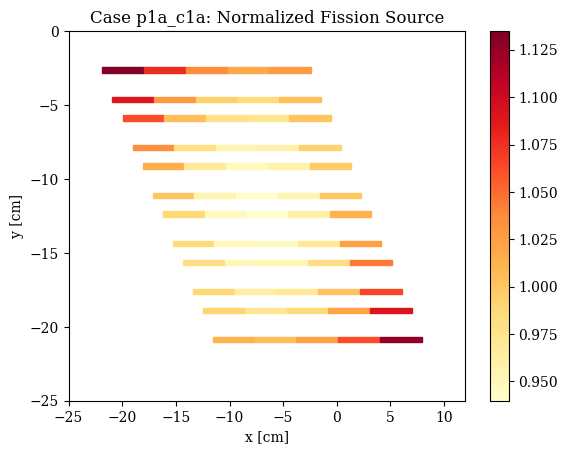
\includegraphics[width=0.49\linewidth]{p1a_c1a_c.png} 
    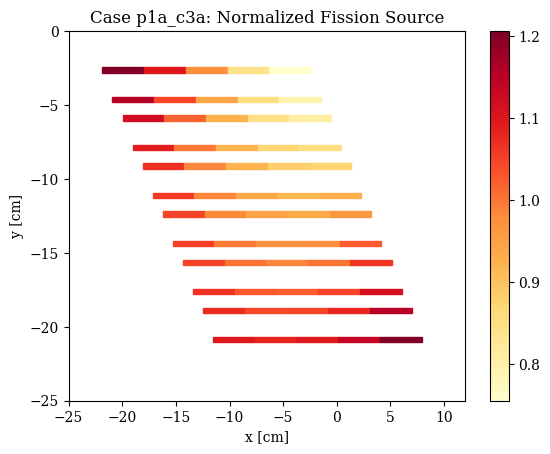
\includegraphics[width=0.49\linewidth]{p1a_c3a_c.png} 
    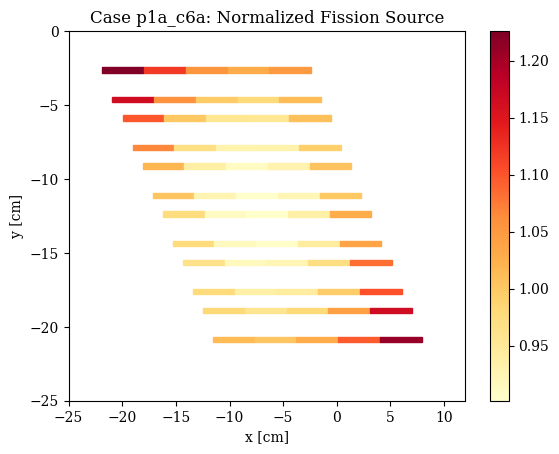
\includegraphics[width=0.49\linewidth]{p1a_c6a_c.png} 
    \caption{\acrlong{UIUC} results: Normalized Fission Source Distribution [-] 
    per one-fifth fuel stripe for \acrlong{FHR} Benchmark's Phase I-A Case 1A 
    (top left), Case 3A (top right), and Case 6A (bottom).}
    \label{fig:phase1a-c}
\end{figure}
Case 4AR has a similar fission source distribution to Case 3A since both 
cases have control rod insertion. 
Case 7A has a similar fission source distribution to case 6A since both have 
higher heavy metal loading. 
All other cases have similar fission source distributions to Case 1A. 

For Case 1A, intuitively, one might assume that the highest fission source would 
occur in the center of the diamond fuel segment; however, the opposite is true. 
Power peaking occurs on exterior stripes and is minimum on the interior stripes.
Gentry et al. \cite{gentry_development_2016} reported similar power peaking 
phenomena towards the lattice cell's exterior closest to the Y-shaped carbon 
support structure.  
This fission source distribution is caused by diminished resonance escape 
probability in the interior due to the higher relative fuel-to-carbon volume 
ratio. 

For Case 3A with an inserted control rod, the fission source is lower in 
the one-fifth stripes closer to the control rod.  
Case 6A demonstrates a further diminished fission source in the interior 
stripes due to the higher fuel-to-carbon ratio.
This is seen in Figure \ref{fig:phase1a-c} in which case 1A and 6A have similar 
fission distribution trends, but case 6A has a bigger fission source value range. 

\subsubsection{Results: Average Neutron Flux (d)}
Figure \ref{fig:phase1a-d} shows the average neutron flux in the fuel assembly in 
three coarse energy groups. 
\begin{figure}[htbp]
    \centering
    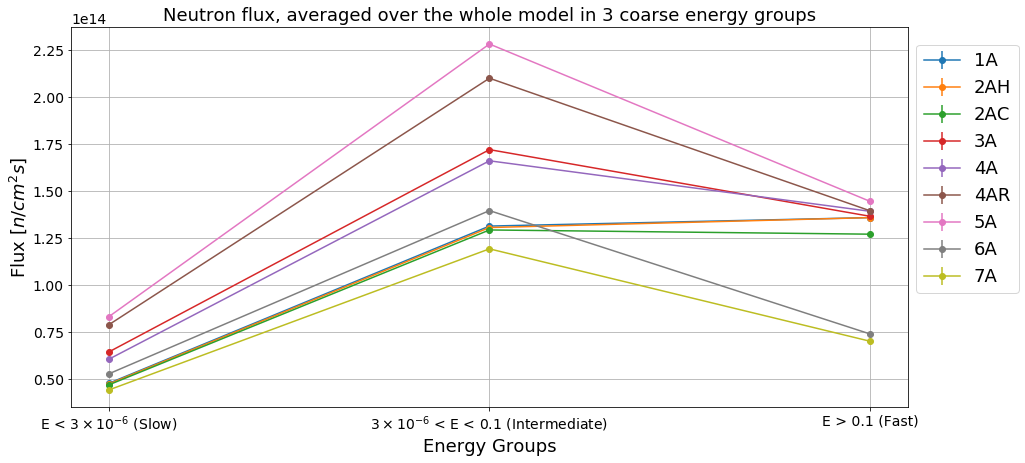
\includegraphics[width=\linewidth]{phase1a-d-flux.png} 
    \caption{\acrlong{UIUC} results: \acrlong{FHR} Benchmark's Neutron flux, 
    averaged over the whole model, tabulated in three coarse energy groups for 
    each Phase I-A case. Neutron flux uncertainty is on the order of 1e10.}
    \label{fig:phase1a-d}
\end{figure}
Most of the cases have the most flux in the intermediate group, followed by 
the thermal group, and the least flux in the fast group.   

\subsubsection{Results: Neutron Flux Distribution (e)}
Figure \ref{fig:phase1a-e} shows the neutron flux distribution in a 100 $\times$ 
100 mesh for Cases 1A, 3A, and 6A for three coarse energy groups. 
\begin{figure}[htbp]
    \centering
    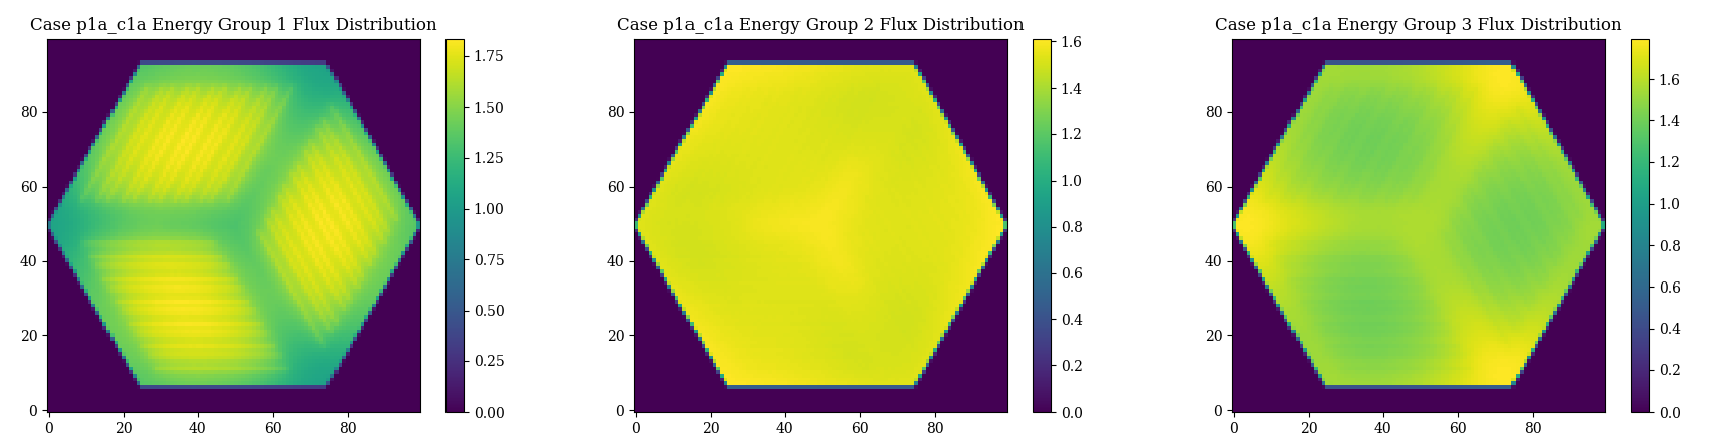
\includegraphics[width=\linewidth]{phase1a-e-c1a.png} 
    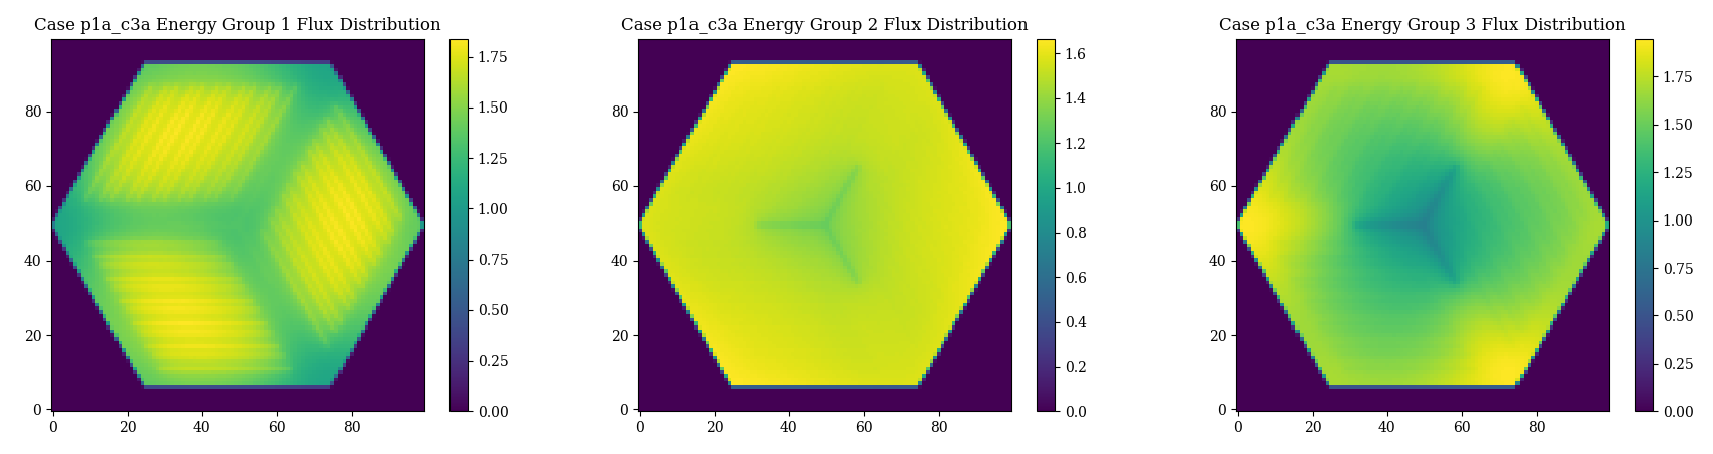
\includegraphics[width=\linewidth]{phase1a-e-c3a.png} 
    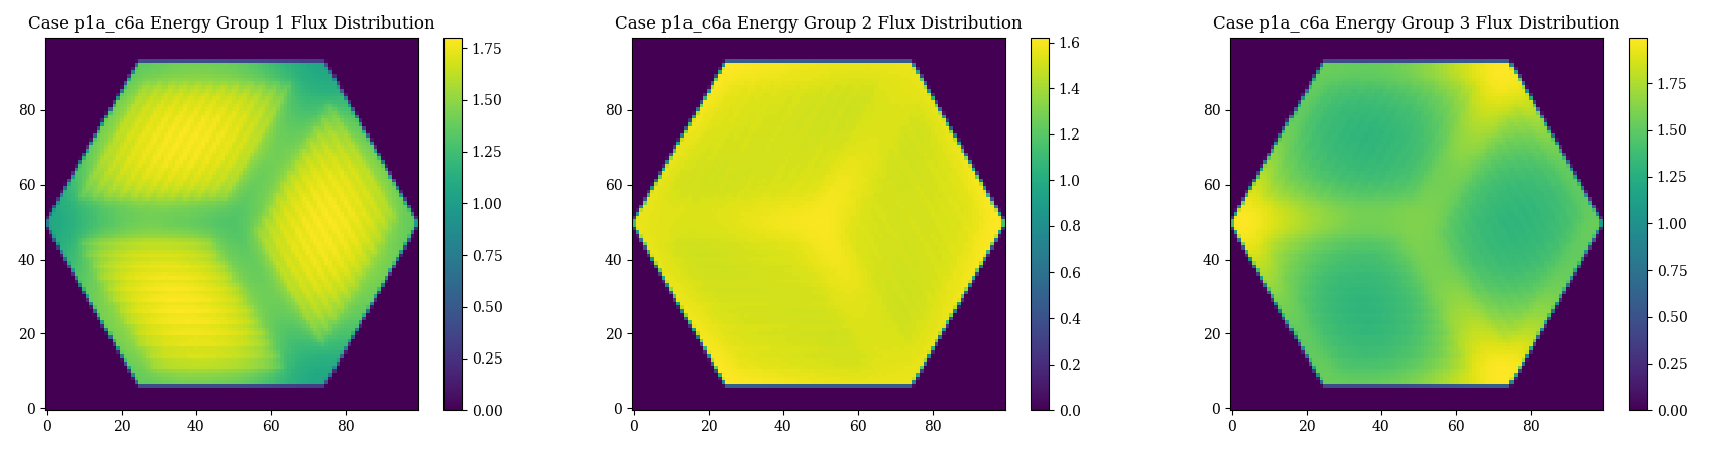
\includegraphics[width=\linewidth]{phase1a-e-c6a.png} 
    \caption{\acrlong{UIUC} results: \acrlong{FHR} Benchmark neutron flux 
    distribution in 100 $\times$ 100 mesh for three coarse energy groups: Case 
    1A (above), Case 3A (middle), Case 6A (below). Energy group 1: $E > 0.1$ MeV, 
    Energy group 2: $3 \times 10^{-6} < E < 0.1$ MeV, Energy group 3: $E < 3 \times 10^{-6}$ MeV. }
    \label{fig:phase1a-e}
\end{figure}
For all three cases, fast-flux (energy group 1) peaks in the diamond-shaped sectors containing 
the fuel stripes, whereas thermal flux (energy group 3) peaks outside of the diamond-shaped 
sectors. 
This can be attributed to fission occurring at thermal energies in the fuel stripe area. 
For Case 3A, the thermal and intermediate neutron flux is depressed in the fuel 
assembly's control rod region.  
An increased heavy metal loading in Case 6A results in a more pronounced 
fast-flux peaking and thermal flux dip in the fuel stripe area. 

\subsubsection{Results: Neutron Spectrum (f)}
Figure \ref{fig:phase1a-f} shows the neutron spectrum for Cases 1A and 6A. 
\begin{figure}[htbp]
    \centering
    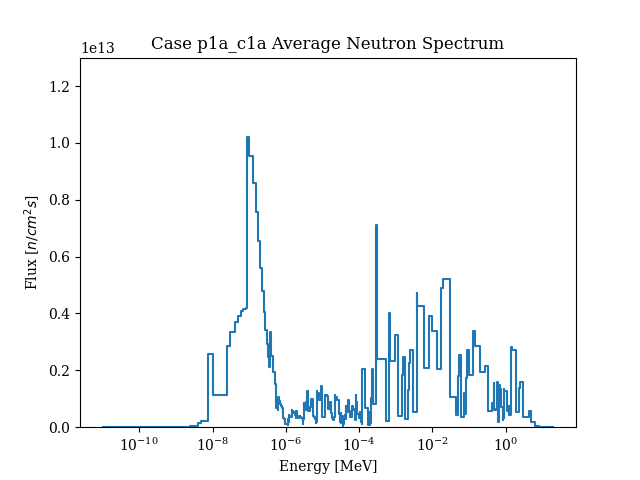
\includegraphics[width=0.49\linewidth]{p1a_c1a_f.png} 
    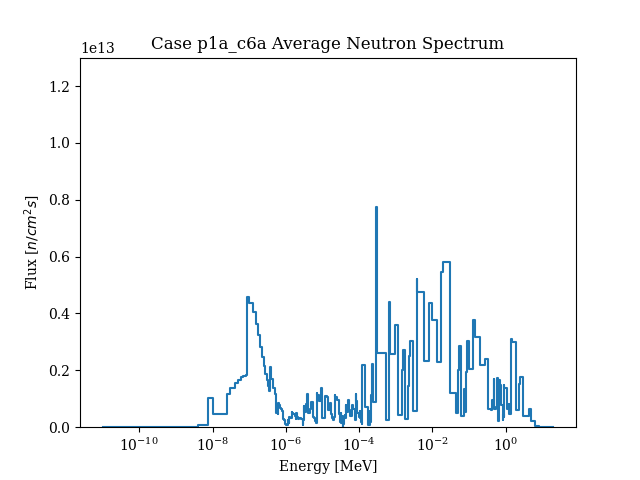
\includegraphics[width=0.49\linewidth]{p1a_c6a_f.png} 
    \caption{\acrlong{UIUC} results: Neutron spectrum for \acrlong{FHR} Benchmark
    Phase I-A Case 1A (left) and Case 6A (right).}
    \label{fig:phase1a-f}
\end{figure}
Case 7A has a similar neutron spectrum to Case 6A since both cases have 
higher fuel content. 
All other cases have a similar neutron spectrum to Case 1A.
The neutron spectra in Cases 6A and 7A are faster due to more heavy metal 
loading and higher enrichment, respectively.  

\subsection{Results: Phase I-B}
Figure \ref{fig:phase1b_keff} shows the $k_{eff}$ evolution during depletion 
for Cases 1B, 4B, and 7B.
\begin{figure}[htbp]
    \centering
    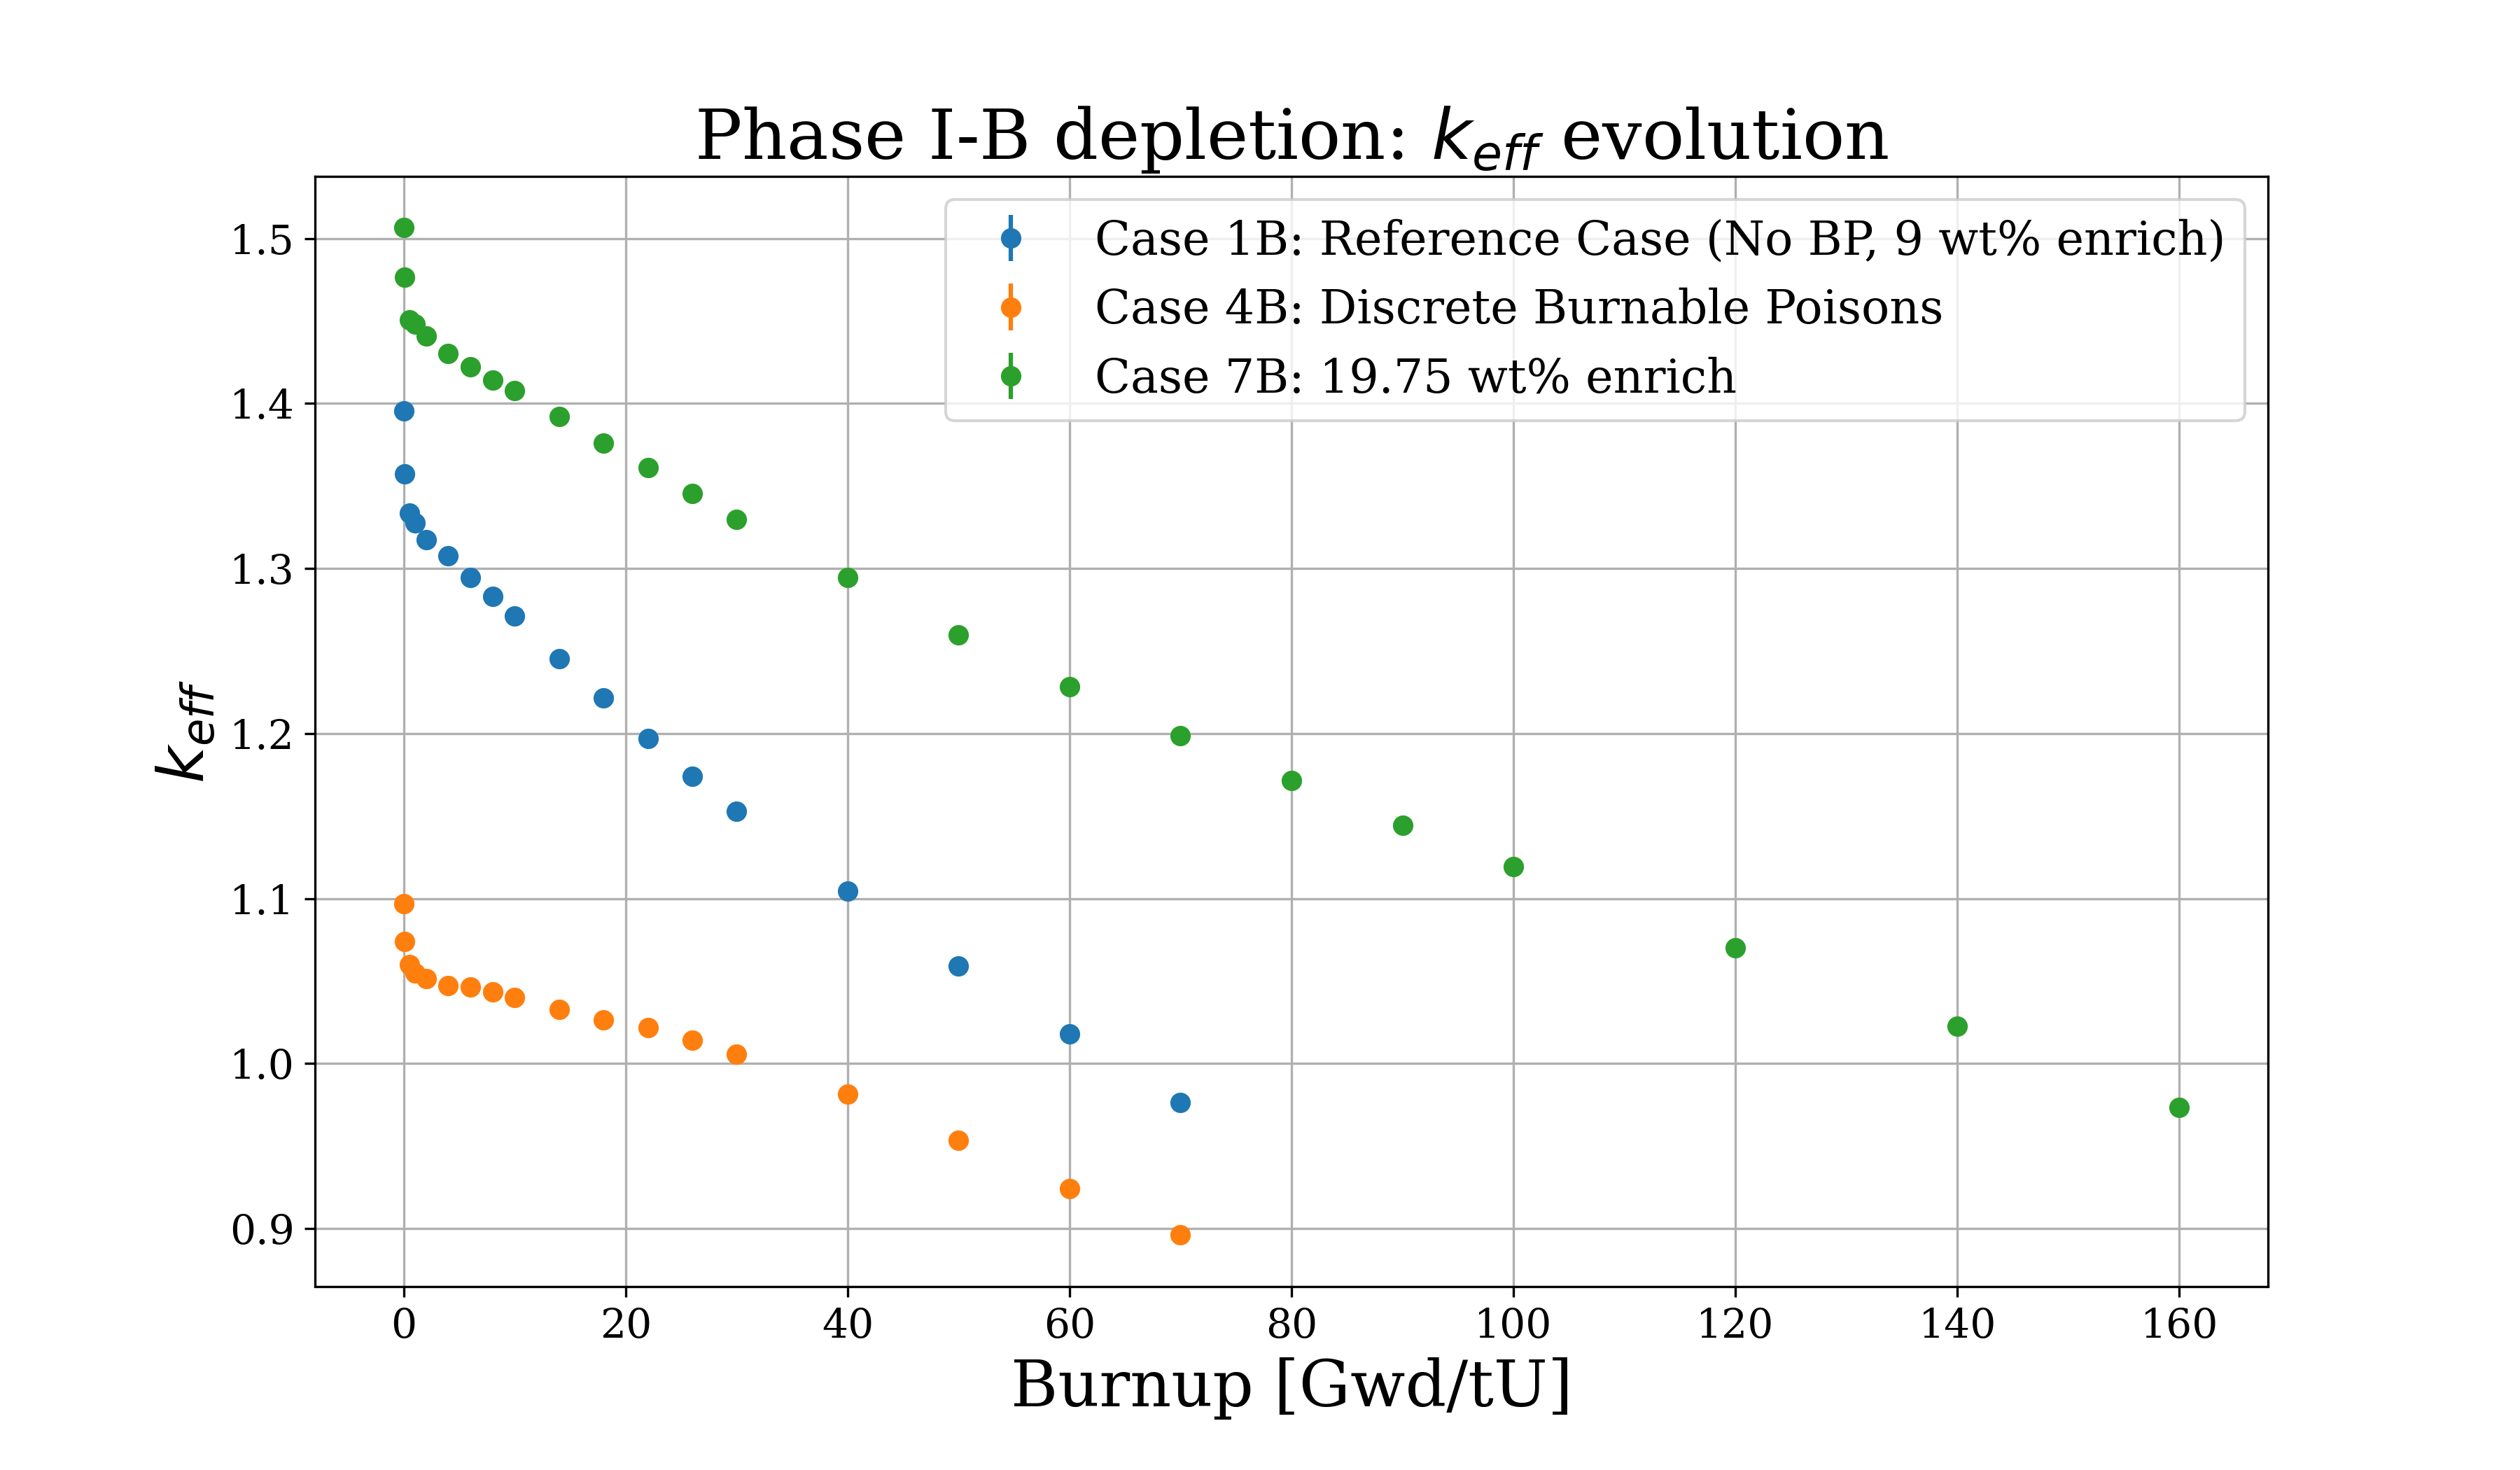
\includegraphics[width=\linewidth]{phase1b_keff.png} 
    \caption{\acrlong{UIUC} results: \acrlong{FHR} Benchmark Phase I-B depletion 
    $k_{eff}$ evolution for Cases 1B, 4B, and 7B. Case 1B is the reference case, 
    Case 4B is the discrete \acrlong{BP} case, and Case 7B is the 19.75$\%$ 
    enrichment case. Error bars are included but are barely visible due to the 
    low $\sim$60pcm uncertainty.}
    \label{fig:phase1b_keff}
\end{figure}
The $k_{eff}$ at zero burnup corresponds to each case's Phase I-A $k_{eff}$ value 
reported in Table \ref{tab:phase1a-results}. 
Case 1B is the reference case with $9\%$ fuel enrichment and no \glspl{BP}. 
Case 1B's $k_{eff}$ steadily decreases until it reaches 0.967845 at the final 70 
GWd/tU burnup. 
Case 4B includes burnable poisons resulting in a lower initial $k_{eff}$. 
Its $k_{eff}$ decreases at a slower rate in the beginning due to the presence of 
burnable poisons, which decreases the flux in the core. 
At approximately 20 GWd/tU, $k_{eff}$ begins decreasing at a faster rate, presumably
due to burn-up of the poison material.   
Case 7B has a $19.75\%$ fuel enrichment, resulting in a higher initial $k_{eff}$. 
With a higher enrichment, the assembly stays critical till 140 Gwd/tU. 

\section{FHR Benchmark Multiphysics Model}
I used Moltres \cite{lindsay_moltres_2017} to conduct \gls{AHTR} full assembly multiphysics 
simulations. 
AHTR Moltres simulations will capture thermal feedback effects, absent from the purely 
neutronics OpenMC simulations conducted in the \gls{FHR} benchmark's Phase I-A.
To run Moltres simulations, the user provides group constant data from a neutron transport 
solver, such as OpenMC, for the Moltres multigroup neutron diffusion calculations and
a mesh file representing the reactor geometry. 
A TRISO-level fidelity mesh file is impractical and will result in an extremely long Moltres 
runtime. 
For successful AHTR Moltres simulation, I must establish suitable spatial and energy 
homogenization that preserves accuracy while maintaining an acceptable runtime.

I use the continuous energy OpenMC simulation to generate multigroup cross section data defined 
over discretized energy groups and spatial segments.
I then use OpenMC's multigroup calculation mode with the previously generated multigroup cross 
section data to calculate $k_{eff}$ . 
Comparison of $k_{eff}$ for the continuous and multigroup simulations determines if the
energy and spatial homogenization used are acceptable.

I modeled the FHR benchmark's Phase I-A hot zero power case 2AH, the OpenMC simulation's 
geometry with TRISO fidelity is shown in Figure \ref{fig:ahtr-fuel-assembly}.
For spatial homogenization of the straightened AHTR fuel assembly, I used OpenMC's \textit{cell} 
domain type to compute multigroup cross sections for different \textit{cells}.
I discretized the fuel assembly into 61 \textit{cells}: inter-assembly \gls{FLiBe}, Y-shaped 
graphite structure, control rod slot \gls{FLiBe}, graphite spacers, each diamond shape section's 
inter-plank \gls{FLiBe} (3), each graphite plank (18), and each fuel stripe (36).

\subsection{FHR Benchmark: Key Neutronics Parameters Verification}
In this section, I verify that the spatial and energy homogenizations I chose are acceptable. 
I compare the following key neutronics parameters: effective multiplication factor, reactivity 
coefficients, flux distribution, and neutron energy spectrum for the OpenMC's continuous energy 
and Moltres' \gls{FHR} benchmark full assembly model. 

\subsubsection{FHR Benchmark: Effective Multiplication Factor}


\subsection{FHR Benchmark: Temperature Model}

\subsubsection{FHR Benchmark: Temperature Model Setup}


\subsubsection{FHR Benchmark: Temperature Model Results}
Figure \ref{fig:benchmark-temperature-model} shows ... 

\section{Summary}